%\documentclass{beamer} %
\documentclass[12pt,handout]{beamer}
\usetheme{CambridgeUS}
\usepackage[utf8]{inputenc}
\usefonttheme{professionalfonts}
\usepackage{times}
\usepackage{tikz}
\usepackage{amsmath}
\usepackage{verbatim}
\usepackage{listings}
\usepackage{hyperref}
\usepackage{yfonts,color}
\usetikzlibrary{arrows,shapes}
\defbeamertemplate{itemize item}{tikzarrow}{\tikz{\node[single
arrow,scale=0.2,inner sep=2ex,fill] at (0,0) {};}}

\lstset{
    language=bash, %% Troque para PHP, C, Java, etc... bash é o padrão
    basicstyle=\ttfamily\small,
    numberstyle=\footnotesize,
    numbers=left,
    backgroundcolor=\color{gray!10},
    frame=single,
    tabsize=2,
    rulecolor=\color{black!30},
    title=\lstname,
    escapeinside={\%*}{*)},
    breaklines=true,
    breakatwhitespace=true,
    framextopmargin=2pt,
    framexbottommargin=2pt,
    inputencoding=utf8,
    extendedchars=true,
    literate={à}{{\`a}}1 {é}{{\'e}}1 {ê}{{\^e}}1,
}

\author{Manuel Martin Infosol}
\title{Vignettes d'un package R (notices)}
\subtitle{Tiré de http://informatique-mia.inra.fr/r4ciam/node/184}

\usepackage{Sweave}
\begin{document}


\begin{frame}
\titlepage
\end{frame}

%-------------------------------------

\begin{frame}[fragile]
\begin{itemize}
\item Il est possible d'intégrer des notices — les "vignettes" dans la terminologie R - aux packages.
\item Les notices d’utilisation des packages R ont intérêt
à être écrites à l'aide de Sweave (et plus récemment de Markdown),
pour que le code et les sorties R soient toujours à jour en cas de modification du package.
\item Ces notices sont par exemples disponibles sur le CRAN \url{https://cran.r-project.org/web/packages/dplyr/index.html}
\end{itemize}
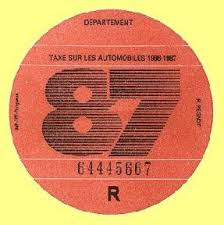
\includegraphics[width = 36pt]{../images/vigtnette.jpg}
\end{frame}

%-------------------------------------

\begin{frame}
\begin{itemize}
\item Le fichier Rnw doit être placé dans le directory vignettes dans la hiérarchie du package.
\item Les commandes "R CMD check" et "R CMD build" génèrent les fichiers TeX et pdf.
\item Pour accéder aux fonctions du package en cours de création, mettre une instruction du type suivant, au sein du code R:
 
\item Pour créer un index de la documentation, insérer une instruction \\VignetteIndexEntry dans un commentaire LaTeX. Exemple :
%\verb!%\VignetteIndexEntry{MONPACKAGE: un package formidable}!
Un fichier index.html sera créé par Sweave.
Il contiendra un lien sur chacun des fichiers pdf, suivi par le libellé choisi dans VignetteIndexEntry.
\end{itemize}

\end{frame}


\end{document}


